The encouraged way to create and edit \PJOB{} files is to use the \pjobeditor\
that is distributed alongside \PHO\ and \PQUEUE.
This section shows how to use this software by presenting a walkthrough for a simple example.


\subsection{Creating a \PJOB\ file}
Using \pjobeditor, creating a valid \PJOB\ file is as easy as issuing the command \textit{File} -\textgreater \textit{New...}
via the application menu or via the shortcut \textbf{CTRL + N} (\textbf{CMD + N} on \mac).
\pjobeditor\ then prompts for the name of the file to be created.
After creating, the file is automatically opened and presented in \pjobeditor's main window
as depicted in figure \ref{editor:new_job_created}.

\begin{figure}[h!]
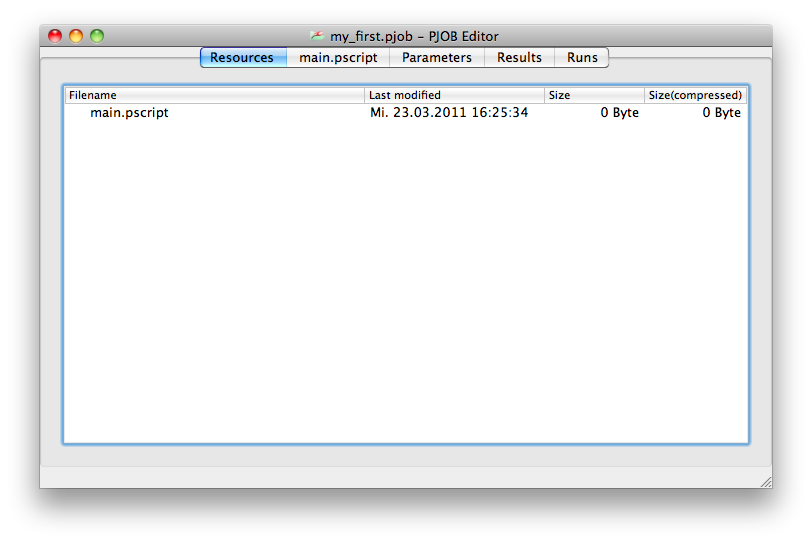
\includegraphics[width=\textwidth]{Screenshots/PJobEditor/new_job_created.png}
\caption{\pjobeditor\ after creating new \PJOB\ file.}
\label{editor:new_job_created}
\end{figure}

It shows multiple tabs from which the \textit{Resource} tab is active.
The resource tab displays the contents of the \PJOB\ file's resource directory
(see section \ref{pjob:structure} \nameref{pjob:structure}) in a tree view.
For a newly created \PJOB\ file, there is only an empty file named \textit{main.pscript}
which is the starting point for the execution of every \PJOB\ file.



\subsection{Adding resources}
By dragging files into this tree view or via the right click context menu,
it is possible to add any number of files or directories to the opened \PJOB\ file.
In order to further describe \pjobeditor's features by example,
suppose we added a directory by right clicking the resources view and choosing \textbf{Make directory},
then renamed that directory to \textit{'PHOs'} by double clicking
and finally added a file called \textit{'my\_system.pho'} to this directory by right clicking the directory
and choosing \textbf{Add resources...} from the context menu
(see figure \ref{editor:pho_added}).

\begin{figure}[h!]
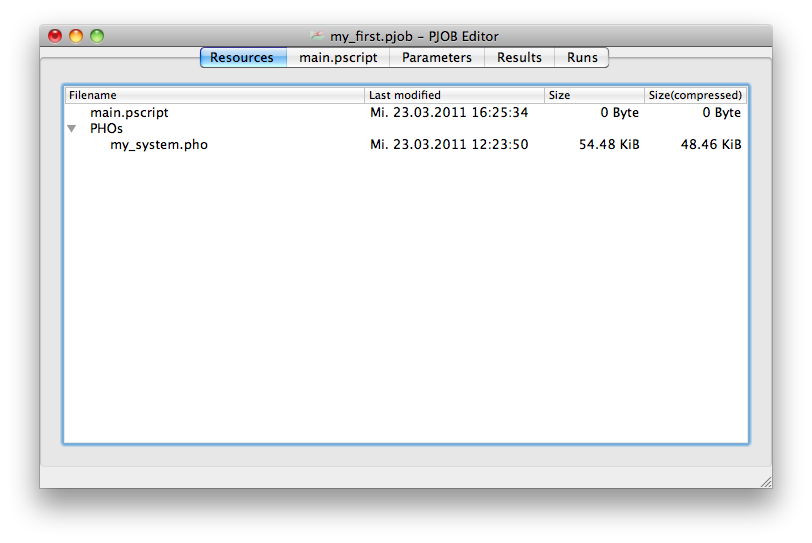
\includegraphics[width=\textwidth]{Screenshots/PJobEditor/pho_added.png}
\caption{\pjobeditor\ after adding a resource file.}
\label{editor:pho_added}
\end{figure}



\subsection{Editing main.pscript}
If we want our \PJOB\ file to actually do something
we have to fill \textit{main.pscript} with \PS\ code.
The simplest example would be to load and run the attached \pho\ file \textit{PHOs/my\_system.pho}.
\PS\ code that accomplishes this would be\footnote{If you are unfamiliar with \PS\
please have a look at the \PS\ manual that is included in this distribution
or see the \PS\ examples which are accessible from \PHO's \PS\ console.}:
\lstset{language=JavaScript, backgroundcolor=\color{gray}, basicstyle=\color{black}}
\begin{lstlisting}
var simulation = Application.openSimulation("PHOs/my_system.pho");
simulation.run();
\end{lstlisting}

It would be possible to write this code into a file in filesystem, rename it to \textit{main.pscript}
and drag it into the \PJOB's resources view, overwriting the empty main.pscript file.
Since editing the \PJOB's behavior is a main use case,
\pjobeditor\ provides support for this task.
\begin{figure}[h!]
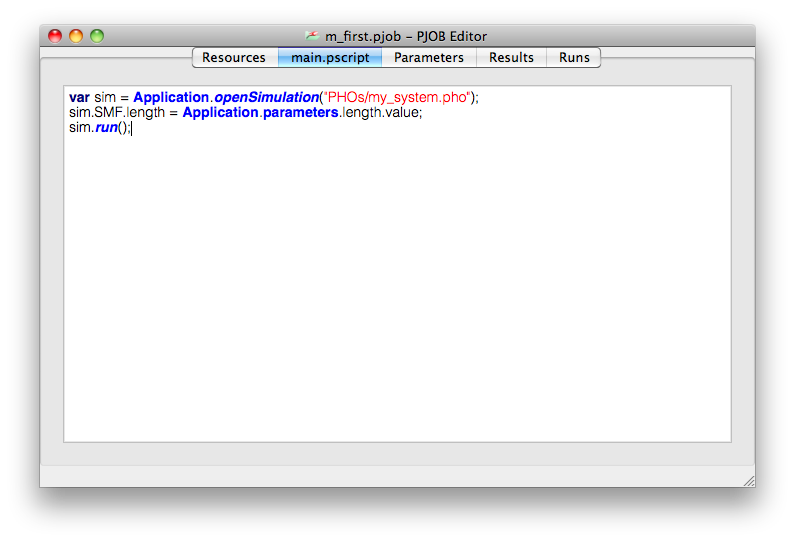
\includegraphics[width=\textwidth]{Screenshots/PJobEditor/main_pscript.png}
\caption{\pjobeditor's main.pscript editor.}
\label{editor:main_pscript}
\end{figure}
Figure \ref{editor:main_pscript} shows the second tab which displays the contents of the \PJOB's main.pscript file
and provides means of editing this file.\bb

Using \PJOB\ files in the context of \PQUEUE,
we would like to parameterize jobs
enabling \PQUEUE\ to distribute calculations of different parameter combinations within the computing grid.
The screenshot shows one additional line:
\begin{lstlisting}
simulation.SMF.length = Application.parameters.length.value;
\end{lstlisting}
This is the \textit{glue code} that takes the \PJOB\ parameter and applies it to the \PJOB's internal structure.
This line implies three facts.
First, there has to be a component named \textit{SMF} within the main network stored in \textit{PHOs/my\_system.pho}.
Furthermore this component needs to have a parameter \textit{length},
what would be expected if this component is of type \textit{Single Mode Fiber}.
Third, the \PJOB file has to declare a parameter named \textit{length}
in order to make \PHO\ add the field \textit{length} to the object \textit{Application.parameters}
when constructing and initializing the script engine that will run this script on execution.
Editing a \PJOB\ file's parameter definitions is also done with \pjobeditor.




\subsection{Editing parameter defintions}
Every parameter of a \PJOB\ has to be declared in order to let \PQUEUE\ know which parameters can be set
and also to make \PHO\ add them to the script context on execution.
As described in section \ref{pjob:parameters},
parameter definitions are stored in an XML file inside the \PJOB\ archive.
You won't have to edit these files manually,
instead \pjobeditor\ provides a GUI editor for parameter definitions within its third tab.
\begin{figure}[h!]
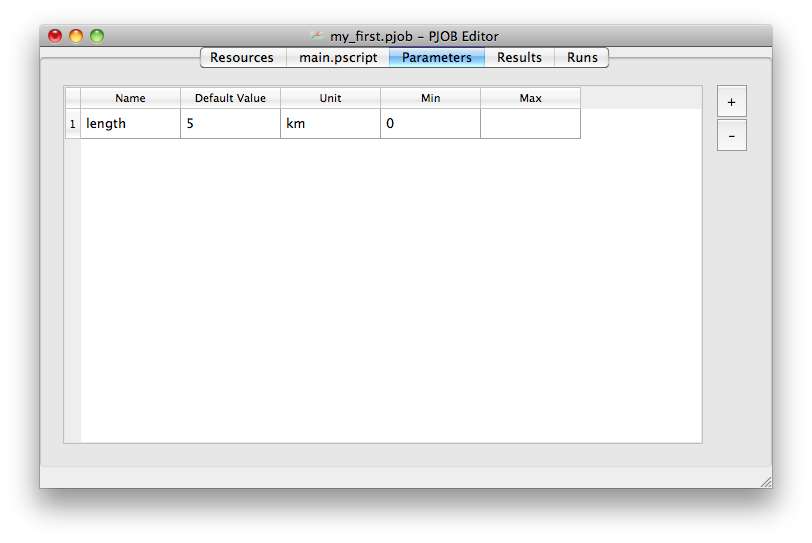
\includegraphics[width=\textwidth]{Screenshots/PJobEditor/parameter.png}
\caption{\pjobeditor's parameter definition editor.}
\label{editor:parameter}
\end{figure}
A new parameter definition is added by clicking the \textit{+} button.
Name, default value and all other properties can be edited by just clicking the appropriate field.
The default value is used by \PHO\ if no value was provided on execution.
\PHO\ makes sure that the \PJOB\ is never executed with parameter values not adhering to the limits set as minimum and maximum value.
Clicking the \textit{-} button removes the selected parameter definition.




\subsection{Editing result definitions}
Depending on the simulation logic implemented in a \PJOB\ file,
results are written to different files and also in different file formats.
In order to let \PQUEUE\ know which file to read results from,
this information has to be stored inside the the \PJOB\ file.
Editing result definitions can be done with \pjobeditor's fourth tab named \textit{Results}.\bb

First, a \textit{result file} has to be added by clicking the \textit{+ result file} button.
Its name has to be changed to the file that is created by \PHO\ or attached scripts on execution.
This has to be a file path relative to the file main.pscript.
Figure \ref{editor:results} shows an example.

\begin{figure}[h!]
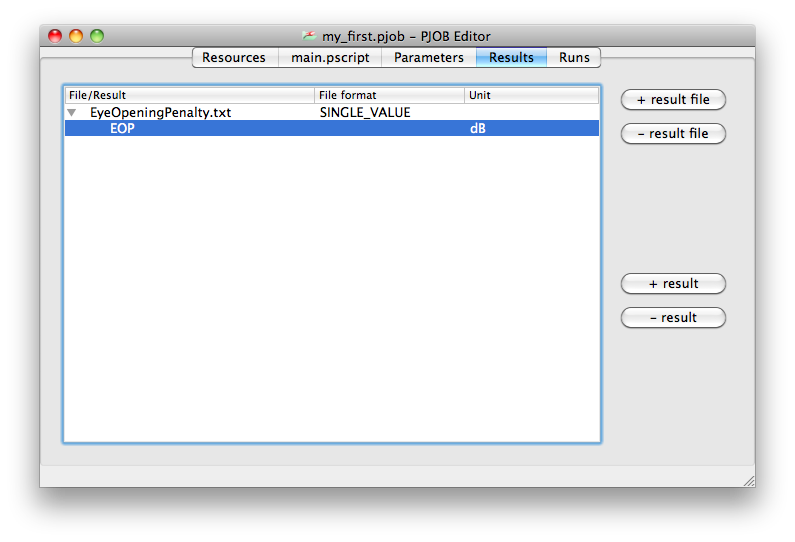
\includegraphics[width=\textwidth]{Screenshots/PJobEditor/results.png}
\caption{\pjobeditor's result definitions editor.}
\label{editor:results}
\end{figure}

The file's format can be set to either \textit{SINGLE\_VALUE} or \textit{CSV}.
For a detailed description on result file formats see section \ref{pjob:results}.
In this case, the result is an ordinary \PHO\ result that is created by the \PHO\ component \textit{Eye Analyzer}.
So this file will contain a single floating point number in text format after execution.
This is exactly what \textit{SINGLE\_VALUE} means.

Only stating the result file's name and format does not suffice.
In case of a \textit{CSV} file, one result file could contain multiple results (and also for multiple parameter combinations).
That is why we have to add a result definition to this result file definition
by clicking the \textit{+ result} button while the result file is selected.
The view now shows an item as the result file's child item.
In case of a \textit{SINGLE\_VALUE} result file,
the name of the result is arbitrary,
but is the name that is used as the result's name within \PQUEUE.
The result's unit can be set by editing the view's third column.
Figure \ref{editor:results_csv} shows an example for a \textit{CSV} result file
as it would be created by \PHO\ when running a parameter variation.
Note that in this case it is mandatory to use the results' names as they are
found in the \textit{CSV} file'as header, i.e. the result names provided by \PHO's components.

\begin{figure}[h!]
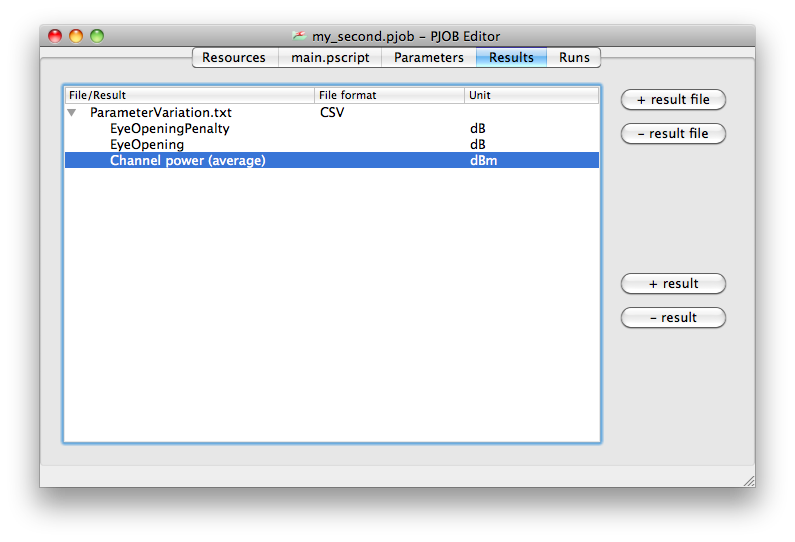
\includegraphics[width=\textwidth]{Screenshots/PJobEditor/results_csv.png}
\caption{\pjobeditor's result definitions for a \textit{CSV} result file.}
\label{editor:results_csv}
\end{figure}




\subsection{Accessing result files}
When executing a \PJOB\ file, \PHO\ adds all created files to a newly created run directory inside the \PJOB\ file.
\pjobeditor\ displays all run directories in it's tree view on tab \textit{Runs}.
Files and folders can be extracted by either dragging them out of this tree view onto the desktop or any other directory
or by right clicking and choosing \textbf{Extract...}.


